\section{Planteamiento del problema}

Se considera una partícula de masa $m$, carga $q$ y espín $s = \frac{1}{2}$
confinada en un pozo unidimensional de longitud $L$:

El potencial $V(x)$ es:
\[
  V(x) = \begin{cases}
    0, & 0 < x < L \\
    \infty, & \text{en otro caso.}
  \end{cases}
\]

El estado físico de la partícula satisface la ecuación de Schrödinger
dependiente del tiempo:
\[
  i\hbar \pdv{\Psi(x,t)}!{t} = \hat{H}\Psi(x(t))
  \quad \text{con} \quad
  \hat{H}=-\frac{\hbar^{2}}{2m} \odv[2]{}!{x} +V(x)
\]

Las soluciones estacionarias son:
\[
  \psi_{n}(x)=\sqrt{\frac{2}{L}}\sin\left(\frac{n\pi x}{L}\right), \quad
  E_{n}=\frac{n^{2}\pi^{2}\hbar^{2}}{2mL^{2}}, \quad n=1,2,3,\ldots
\]

Se sabe que la partícula puede estar en una superposición lineal de
estos estados estacionarios antes de ser medida:
\[
  \ket{\psi} = \alpha \ket{n=1} + \beta \ket{n=2},
\]
donde $|\alpha|^{2}+|\beta|^{2}=1$.

A partir de este punto, se pide construir de manera progresiva la descripción
lógica y computacional cuántica de este sistema.

\section{Revisión conceptual del sistema físico}

\subsection{Funciones de onda normalizadas}

Las funciones de onda normalizadas para los dos primeros estados estacionarios
($n=1$ y $n=2$) son:
\[
  \psi_{1}(x) = \sqrt{\frac{2}{L}}\sin\left(\frac{\pi x}{L}\right)
\]
\[
  \psi_{2}(x) = \sqrt{\frac{2}{L}}\sin\left(\frac{2\pi x}{L}\right)
\]

Comprobamos que las funciones de onda $\psi_n(x)$ están normalizadas dentro del
dominio $[0, L]$.
\begin{align*}
  \langle\psi_{n}|\psi_{n}\rangle &= \int_{0}^{L}\psi_{n}^{*}(x)\psi_{n}(x)dx
  = \int_{0}^{L}\left(\sqrt{\frac{2}{L}}\sin\left(\frac{n\pi x}{L}\right)\right)^{2} dx \\
                                  &= \frac{2}{L}\int_{0}^{L}\sin^{2}\left(\frac{n\pi x}{L}\right)dx
\end{align*}
Recordando la identidad trigonométrica $\sin^{2}\theta=\frac{1}{2}(1-\cos(2\theta))$:
\begin{align*}
  \langle\psi_{n}|\psi_{n}\rangle &= \frac{2}{L}\int_{0}^{L}\frac{1}{2}\left[1-\cos\left(\frac{2n\pi x}{L}\right)\right]dx \\
                                  &= \frac{1}{L}\left[\int_{0}^{L}dx - \int_{0}^{L}\cos\left(\frac{2n\pi x}{L}\right)dx\right] \\
                                  &= \frac{1}{L}\left[ [x]_{0}^{L} - \left[\frac{L}{2n\pi}\sin\left(\frac{2n\pi x}{L}\right)\right]_{0}^{L} \right] \\
                                  &= \frac{1}{L}\left[ (L-0) - \left(\frac{L}{2n\pi}\sin(2n\pi) - \frac{L}{2n\pi}\sin(0)\right) \right] \\
                                  &= \frac{1}{L}\left[ L - (0 - 0) \right] = 1
\end{align*}
Por ende, las funciones $\psi_n(x)$ están normalizadas.

\subsection{Verificación de Ortogonalidad}

Verificamos la ortogonalidad para dos estados distintos $n \neq m$. En
particular, para $n=1$ y $m=2$.
\begin{align*}
  \langle\psi_{n}|\psi_{m}\rangle &= \int_{0}^{L}\psi_{n}^{*}(x)\psi_{m}(x)dx
  = \frac{2}{L}\int_{0}^{L}\sin\left(\frac{n\pi x}{L}\right)\sin\left(\frac{m\pi x}{L}\right)dx
\end{align*}
Usando la identidad $\sin(a)\sin(b) = \frac{1}{2}[\cos(a-b)-\cos(a+b)]$:
\begin{align*}
  \langle\psi_{n}|\psi_{m}\rangle &= \frac{2}{L} \int_{0}^{L} \frac{1}{2}\left[ \cos\left(\frac{\pi x}{L}(n-m)\right) - \cos\left(\frac{\pi x}{L}(n+m)\right) \right]dx \\
                                  &= \frac{1}{L} \left[ \frac{L}{\pi(n-m)}\sin\left(\frac{\pi x}{L}(n-m)\right) - \frac{L}{\pi(n+m)}\sin\left(\frac{\pi x}{L}(n+m)\right) \right]_{0}^{L} \\
                                  &= \frac{1}{\pi(n-m)}\left[\sin(\pi(n-m)) - \sin(0)\right] - \frac{1}{\pi(n+m)}\left[\sin(\pi(n+m)) - \sin(0)\right]
\end{align*}
Dado que $n$ y $m$ son enteros distintos, $(n-m)$ y $(n+m)$ son enteros. El seno de cualquier múltiplo entero de $\pi$ (como $\sin(\pi(n-m))$) es cero.
\[
  \langle\psi_{n}|\psi_{m}\rangle = 0 - 0 = 0 \quad (\text{para } n \neq m)
\]
Específicamente para $n=1$ y $m=2$:
\[
  \langle\psi_{1}|\psi_{2}\rangle = 0
\]

\subsection{Interpretación física de la Ortogonalidad}

La ortogonalidad $\langle\psi_1|\psi_2\rangle = 0$ implica consecuencias físicas
fundamentales para la medición:
\begin{itemize}
  \item \textbf{Distinguibilidad Perfecta:} Los estados ortogonales son
    perfectamente distinguibles. Si preparamos un estado que es $\psi_1$ o
    $\psi_2$, una sola medición de un observable apropiado (como la energía)
    puede determinar con certeza cuál de los dos estados era.

  \item \textbf{Proyectores de Medida:} Estos estados ortogonales definen
    proyectores de medida asociados a cada autoestado, dados por $P_n =
    |\psi_n\rangle\langle\psi_n|$. Estos proyectores cumplen la propiedad $P_n
    P_m = 0$ para $n \neq m$, lo que matemáticamente refuerza la idea de que los
    resultados son mutuamente excluyentes.

  \item \textbf{Mediciones Mutuamente Excluyentes:} Si el sistema está en el
    estado $\psi_1$, la probabilidad de medir el valor de energía $E_2$
    (asociado a $\psi_2$) es cero, y viceversa. La ortogonalidad implica que
    estos resultados son mutuamente excluyentes.

  \item \textbf{Base para Codificar Información:} Esta estructura ortogonal es
    óptima para la codificación de información binaria. Al elegir $\psi_1$ y
    $\psi_2$ como nuestros estados base, podemos representar los dos posibles
    estados de un sistema binario. La ventaja es que el sistema permite
    mediciones sin ambigüedad (100\% distinguibles).
\end{itemize}
\section{Definición de la base lógica}

Aquí se formaliza la elección de los estados estacionarios como la base lógica
(o computacional) de un qubit, basándose en lo encontrado en la sección
anterior.

\subsection{Definición de estados lógicos}

Se definen los estados de la base computacional (o lógica) utilizando los dos
primeros autoestados de energía del sistema:
\[
  |0_L\rangle \equiv |\psi_1\rangle
\]
\[
  |1_L\rangle \equiv |\psi_2\rangle
\]
Se denota $\mathcal{H}_L$ al subespacio de Hilbert generado por estos dos
vectores base:
\[
  \mathcal{H}_L = \text{span}\{|\psi_1\rangle, |\psi_2\rangle\} = \text{span}\{|0_L\rangle, |1_L\rangle\}
\]

\subsection{Demostración de Base Ortonormal}

Para demostrar que el conjunto $\{|0_L\rangle, |1_L\rangle\}$ forma una base
ortonormal para el subespacio $\mathcal{H}_L$, debemos probar dos condiciones:
ortonormalidad e independencia lineal.

\subsubsection*{Ortonormalidad}
Como se demostró en la Sección 1, los estados $\psi_1$ y $\psi_2$ son
ortonormales. Por lo tanto, por definición:
\begin{itemize}
  \item Normalidad: $\langle 0_L|0_L\rangle = \langle\psi_1|\psi_1\rangle = 1$ y $\langle 1_L|1_L\rangle = \langle\psi_2|\psi_2\rangle = 1$.
  \item Ortogonalidad: $\langle 0_L|1_L\rangle = \langle\psi_1|\psi_2\rangle = 0$.
\end{itemize}
El conjunto es ortonormal.

\subsubsection*{Independencia Lineal}
Para probar la independencia lineal, tomamos una combinación lineal de los vectores base igualada al vector cero:
\[
  a|0_L\rangle + b|1_L\rangle = 0 \quad \text{donde } a, b \in \mathbb{C}
\]
Para que sean linealmente independientes, debemos demostrar que la única solución es $a=0$ y $b=0$.

Aplicamos el bra $\langle 0_L|$ por la izquierda:
\begin{align*}
  \langle 0_L| (a|0_L\rangle + b|1_L\rangle) &= \langle 0_L|0\rangle \\
  a\langle 0_L|0_L\rangle + b\langle 0_L|1_L\rangle &= 0 \\
  a(1) + b(0) &= 0 \\
  a &= 0
\end{align*}
Ahora, aplicamos el bra $\langle 1_L|$ por la izquierda:
\begin{align*}
  \langle 1_L| (a|0_L\rangle + b|1_L\rangle) &= \langle 1_L|0\rangle \\
  a\langle 1_L|0_L\rangle + b\langle 1_L|1_L\rangle &= 0 \\
  a(0) + b(1) &= 0 \\
  b &= 0
\end{align*}
Dado que la única solución es $a=0$ y $b=0$, los vectores son linealmente independientes.

Al ser un conjunto de dos vectores linealmente independientes y ortonormales, forman una base para el subespacio de dimensión 2 que generan ($\mathcal{H}_L$).

\subsection{Interpretación como Qubit Lógico e Implicaciones}

Interpretar esta base como la de un qubit lógico es el paso fundamental que conecta la mecánica cuántica del pozo con la computación cuántica. Las implicaciones de esta elección son:

\begin{itemize}
  \item \textbf{Sistema Efectivo de 2 Niveles (Qubit):} Al restringir el análisis al subespacio $\mathcal{H}_L$, el sistema físico (que tiene infinitos niveles) se trata como un sistema binario efectivo. Esta es la unidad básica de información cuántica, el qubit lógico. Un estado general del qubit es una superposición $|\psi\rangle = \alpha|0_L\rangle + \beta|1_L\rangle$.

  \item \textbf{Medición y Regla de Born:} El postulado de la medida se aplica a esta base. Si el sistema está en el estado $|\psi\rangle$, al medir en la base lógica (que físicamente corresponde a medir la energía), la probabilidad de obtener el resultado $E_1$ (estado $|0_L\rangle$) es $P(0) = |\langle 0_L|\psi\rangle|^2 = |\alpha|^2$, y la probabilidad de obtener $E_2$ (estado $|1_L\rangle$) es $P(1) = |\langle 1_L|\psi\rangle|^2 = |\beta|^2$.

  \item \textbf{Limitaciones Físicas (Fuga):} Esta es una idealización. El
    sistema físico real posee otros niveles ($n=3, 4, \dots$). Una implicación
    crucial es que cualquier operación física sobre el qubit debe diseñarse
    cuidadosamente para no ``excitar'' la partícula a estos niveles superiores,
    lo que se conoce como \emph{fuga} (leakage). El sistema debe permanecer dentro del subespacio $\mathcal{H}_L$.

  \item \textbf{Operaciones Unitarias (Puertas Lógicas):} La dinámica del qubit (las puertas lógicas) debe ser implementada mediante operaciones unitarias $U$ que dejen el subespacio $\mathcal{H}_L$ invariante ($U: \mathcal{H}_L \to \mathcal{H}_L$). Físicamente, esto exige la construcción de campos o perturbaciones externas que provoquen transiciones controladas solo entre $|\psi_1\rangle$ y $|\psi_2\rangle$, sin afectar a otros estados.
\end{itemize}
\section{Estado antes de la medición}

\subsection{Estado en la representación de posición}

El estado general del qubit en el subespacio lógico $\mathcal{H}_L$ es:
\[
  |\psi\rangle = \alpha|0_L\rangle + \beta|1_L\rangle
\]
Usando la definición de la base lógica ($|0_L\rangle \equiv |\psi_1\rangle$ y
$|1_L\rangle \equiv |\psi_2\rangle$), reescribimos el estado en términos de los
autoestados de energía:
\[
  |\psi\rangle = \alpha|\psi_1\rangle + \beta|\psi_2\rangle
\]
La representación en la base de posición $\Psi(x)$ se obtiene proyectando este
estado sobre el bra $\langle x|$:
\begin{align*}
  \Psi(x) &= \langle x | \psi \rangle \\
          &= \langle x | (\alpha|\psi_1\rangle + \beta|\psi_2\rangle) \\
          &= \alpha\langle x|\psi_1\rangle + \beta\langle x|\psi_2\rangle \\
          &= \alpha\psi_1(x) + \beta\psi_2(x)
\end{align*}
Sustituyendo explícitamente las funciones de onda normalizadas:
\[
  \Psi(x) = \alpha\sqrt{\frac{2}{L}}\sin\left(\frac{\pi x}{L}\right) +
  \beta\sqrt{\frac{2}{L}}\sin\left(\frac{2\pi x}{L}\right)
\]

\subsection{Cálculo de \texorpdfstring{$|\Psi(x)|^2$}{|Ψ(x)|²} y Términos de Interferencia}

La densidad de probabilidad de encontrar la partícula en la posición $x$ se
calcula como $|\Psi(x)|^2 = \Psi^*(x)\Psi(x)$. Asumiendo que las funciones de
onda $\psi_n(x)$ son reales, pero los coeficientes $\alpha$ y $\beta$ pueden ser
complejos:
\begin{align*}
  |\Psi(x)|^2 &= (\alpha^*\psi_1(x) + \beta^*\psi_2(x)) (\alpha\psi_1(x) + \beta\psi_2(x)) \\
              &= \alpha^*\alpha \psi_1(x)^2 + \beta^*\beta \psi_2(x)^2 + \alpha^*\beta \psi_1(x)\psi_2(x) + \beta^*\alpha \psi_1(x)\psi_2(x) \\
              &= |\alpha|^2 \psi_1(x)^2 + |\beta|^2 \psi_2(x)^2 + (\alpha^*\beta + \beta^*\alpha) \psi_1(x)\psi_2(x)
\end{align*}
El término $(\alpha^*\beta + \beta^*\alpha)$ es igual a $2 \text{Re}(\alpha^*\beta)$. Por lo tanto:
\[
  |\Psi(x)|^2 = \underbrace{|\alpha|^2 |\psi_1(x)|^2}_{\text{Prob. estado 1}} +
  \underbrace{|\beta|^2 |\psi_2(x)|^2}_{\text{Prob. estado 2}} + \underbrace{2
  \text{Re}(\alpha^*\beta) \psi_1(x)\psi_2(x)}_{\textbf{Término de
Interferencia}}
\]

\textbf{Discusión de la interferencia:}

Al analizar la densidad de probabilidad $|\Psi(x)|^2$, se observa que los dos
primeros términos representan la suma de las densidades de probabilidad
individuales para cada estado, ponderadas por sus respectivas probabilidades
($|\alpha|^2$ y $|\beta|^2$). Sin embargo, a diferencia de lo que ocurriría en
un sistema no cuántico, aparece un tercer término, conocido como el ``término de
interferencia cuántica'', el cual es un resultado directo del principio de
superposición. El valor de este término depende crucialmente tanto del producto
de \textit{ambas} funciones de onda, $\psi_1(x)\psi_2(x)$, como de la relación
de fase relativa entre los coeficientes $\alpha$ y $\beta$ (contenida en la
expresión $\text{Re}(\alpha^*\beta)$). Dependiendo de la posición $x$ y de esta
fase, el término de interferencia puede ser positivo (interferencia
constructiva) o negativo (interferencia destructiva), modificando la densidad de
probabilidad total de formas no clásicas.

\subsection{Observable físico de la base lógica}

Se analiza a continuación qué observable físico corresponde a una medición en la
base lógica $\{|0_L\rangle, |1_L\rangle\}$. Por definición, esta base se ha
construido a partir de los estados estacionarios del pozo de potencial:
$|0_L\rangle \equiv |\psi_1\rangle$ y $|1_L\rangle \equiv |\psi_2\rangle$. Los
estados estacionarios $\psi_n$ son, por definición, los autoestados
(eigenstates) del operador Hamiltoniano $\hat{H}$ del sistema. Esto implica que
los estados de nuestra base lógica tienen autovalores (eigenvalues) de energía
definidos, tal como lo muestran las ecuaciones:
\[
  \hat{H}|0_L\rangle = \hat{H}|\psi_1\rangle = E_1|\psi_1\rangle = E_1|0_L\rangle
\]
\[
  \hat{H}|1_L\rangle = \hat{H}|\psi_2\rangle = E_2|\psi_2\rangle = E_2|1_L\rangle
\]
Por lo tanto, el observable físico que corresponde a una medición en la base
computacional $\{|0_L\rangle, |1_L\rangle\}$ es la energía del sistema. Realizar
una ``medición computacional'' en este qubit es físicamente equivalente a medir
la energía de la partícula. Si el resultado de la medición es $E_1$ (lo cual
ocurre con probabilidad $|\alpha|^2$), el estado ha colapsado a $|0_L\rangle$;
si el resultado es $E_2$ (con probabilidad $|\beta|^2$), el estado ha colapsado
a $|1_L\rangle$.
\section{Inclusión del espín y carga}

\subsection{Espacio de estados total (Producto Tensorial)}

El estado de la partícula no solo se describe por su posición (o nivel de
energía), sino también por su espín. Para describir el estado completo, debemos
combinar el espacio de estados de la parte espacial (nuestro qubit lógico) con
el espacio de estados del espín.

El espacio de estados total $\mathcal{H}_{total}$ es el producto tensorial del
subespacio lógico $\mathcal{H}_L$ (al que nos hemos restringido) y el espacio de
espín $\mathcal{H}_{spin}$:
\[
  \mathcal{H}_{total} = \mathcal{H}_{L} \otimes \mathcal{H}_{spin}
\]
Donde:
\begin{itemize}
  \item $\mathcal{H}_L = \text{span}\{|0_L\rangle, |1_L\rangle\}$ es el espacio
    de 2 dimensiones del qubit lógico (energía).
  \item $\mathcal{H}_{spin} = \text{span}\{|\uparrow\rangle,
    |\downarrow\rangle\}$ es el espacio de 2 dimensiones del espín $s=1/2$.
\end{itemize}
El espacio total resultante $\mathcal{H}_{total}$ es, por lo tanto, un espacio
de $2 \times 2 = 4$ dimensiones. La base de este espacio está formada por todas
las combinaciones posibles:
\[
  \{ |0_L\rangle \otimes |\uparrow\rangle, \quad |0_L\rangle \otimes
    |\downarrow\rangle, \quad |1_L\rangle \otimes |\uparrow\rangle, \quad
  |1_L\rangle \otimes |\downarrow\rangle \}
\]

A menudo, esto se abrevia como $\{ |0_L \uparrow\rangle, |0_L \downarrow\rangle,
|1_L \uparrow\rangle, |1_L \downarrow\rangle \}$

\subsection{Significado físico del Producto Tensorial}

El producto tensorial $\otimes$ es la herramienta matemática que nos permite
describir estados de sistemas compuestos o de un solo sistema con múltiples
grados de libertad (como en este caso, posición y espín).

\textbf{Significado Físico:} Un estado en $\mathcal{H}_{total}$ debe especificar
\textit{simultáneamente} la información de ambas partes. El producto tensorial
nos dice que el estado de la partícula es una combinación (ya sea separable o
entrelazada) de un estado en $\mathcal{H}_L$ y un estado en
$\mathcal{H}_{spin}$.

\textbf{Ejemplo Explícito:}
El estado que se propone es:
\[
  |\Psi\rangle = |0_L\rangle \otimes | \uparrow\rangle
\]
Este es un \textit{estado separable}. Su interpretación física es clara:
\begin{itemize}
  \item La partícula se encuentra en el estado de energía $E_1$ (correspondiente
    al estado lógico $|0_L\rangle$).
  \item Y, al mismo tiempo, su espín está en el estado ``arriba''
    ($|\uparrow\rangle$).
\end{itemize}
Un estado general en este espacio será una superposición de los 4 estados base,
lo que permite también la existencia de \textit{estados entrelazados} (no
separables) entre el espacio y el espín, como por ejemplo
$\frac{1}{\sqrt{2}}(|0_L \uparrow\rangle + |1_L \downarrow\rangle)$.

\subsection{Nuevos grados de libertad y efectos de la carga}

\subsubsection*{Nuevos Grados de Libertad (Espín)}
El espín añade un nuevo grado de libertad binario. Antes, nuestro sistema (el
qubit lógico $\mathcal{H}_L$) era un sistema de 2 niveles. Al incluir el espín,
el sistema completo $\mathcal{H}_{total}$ se convierte en un sistema de 4
niveles.

Esta inclusión tiene implicaciones físicas significativas:
\begin{enumerate}
  \item \textbf{Más información:} El sistema ahora puede almacenar dos qubits de
    información (uno en la energía/posición y otro en el espín).
  \item \textbf{Nuevas interacciones:} Se pueden diseñar interacciones que
    actúen selectivamente sobre la parte espacial o sobre la parte de espín.
  \item \textbf{Entrelazamiento:} Como se mencionó, permite la creación de
    entrelazamiento entre las propiedades espaciales y de espín de la
    \textit{misma} partícula.
\end{enumerate}

\subsubsection*{Efectos de la Carga Eléctrica ($q$)}
La carga y el espín hacen que la partícula sea sensible a los campos
electromagnéticos, lo cual es fundamental para su \textit{control}:
\begin{itemize}
  \item \textbf{Efecto de un Campo Eléctrico ($\vec{E}$):} La carga $q$
    interactuará con un campo eléctrico (p.ej., $\hat{V}_{E} =
    -q\vec{E}\cdot\vec{x}$). Un campo eléctrico puede usarse para modular el
    potencial del pozo $V(x)$, por ejemplo, ``inclinándolo''. Esto modificaría
    las funciones de onda $\psi_1, \psi_2$ y sus energías $E_1, E_2$. Un campo
    eléctrico permitiría, por tanto, controlar el qubit lógico espacial (p.ej.,
    inducir transiciones entre $|0_L\rangle$ y $|1_L\rangle$).

  \item \textbf{Efecto de un Campo Magnético ($\vec{B}$):} La partícula, al
    tener espín $s=1/2$, posee un momento dipolar magnético $\vec{\mu}$. Este
    momento magnético interactuará con un campo magnético externo $\vec{B}$ a
    través del término de Zeeman ($\hat{H}_{Z} \approx -\vec{\mu} \cdot
    \vec{B}$). Esta interacción afecta principalmente a los estados de espín
    ($|\uparrow\rangle$ y $|\downarrow\rangle$), rompiendo su degeneración en
    energía. Por lo tanto, un campo magnético (especialmente uno oscilante)
    permitiría controlar el qubit de espín.
\end{itemize}
\section{Observables de Pauli en el subespacio lógico}
\label{sec:observables_pauli}

En esta sección, se definen los operadores análogos a las matrices de Pauli,
pero que actúan exclusivamente dentro del subespacio lógico de 2D,
$\mathcal{H}_L$.

\subsection{Definición y Representación Matricial}

Los operadores de Pauli en la base lógica $\{|0_L\rangle, |1_L\rangle\}$ se
definen como:
\begin{align*}
  X_L &= |0_L\rangle\langle 1_L| + |1_L\rangle\langle 0_L| \\
  Y_L &= -i|0_L\rangle\langle 1_L| + i|1_L\rangle\langle 0_L| \\
  Z_L &= |0_L\rangle\langle 0_L| - |1_L\rangle\langle 1_L|
\end{align*}

Para encontrar sus representaciones matriciales, usamos la correspondencia de
los vectores base:
\[
  |0_L\rangle \to \begin{pmatrix} 1 \\ 0 \end{pmatrix} \quad \text{y} \quad |1_L\rangle \to \begin{pmatrix} 0 \\ 1 \end{pmatrix}
\]
Y los operadores (proyectores externos) correspondientes:
\begin{align*}
  |0_L\rangle\langle 0_L| &\to \begin{pmatrix} 1 \\ 0 \end{pmatrix} \begin{pmatrix} 1 & 0 \end{pmatrix} = \begin{pmatrix} 1 & 0 \\ 0 & 0 \end{pmatrix} \\
  |1_L\rangle\langle 1_L| &\to \begin{pmatrix} 0 \\ 1 \end{pmatrix} \begin{pmatrix} 0 & 1 \end{pmatrix} = \begin{pmatrix} 0 & 0 \\ 0 & 1 \end{pmatrix} \\
  |0_L\rangle\langle 1_L| &\to \begin{pmatrix} 1 \\ 0 \end{pmatrix} \begin{pmatrix} 0 & 1 \end{pmatrix} = \begin{pmatrix} 0 & 1 \\ 0 & 0 \end{pmatrix} \\
  |1_L\rangle\langle 0_L| &\to \begin{pmatrix} 0 \\ 1 \end{pmatrix} \begin{pmatrix} 1 & 0 \end{pmatrix} = \begin{pmatrix} 0 & 0 \\ 1 & 0 \end{pmatrix}
\end{align*}

Sustituyendo estos en las definiciones, obtenemos las representaciones
matriciales (que coinciden con las matrices de Pauli estándar, $\sigma_x,
\sigma_y, \sigma_z$):

\[
  X_L \to \begin{pmatrix} 0 & 1 \\ 0 & 0 \end{pmatrix} + \begin{pmatrix} 0 & 0 \\ 1 & 0 \end{pmatrix} = \begin{pmatrix} 0 & 1 \\ 1 & 0 \end{pmatrix}
\]
\[
  Y_L \to -i\begin{pmatrix} 0 & 1 \\ 0 & 0 \end{pmatrix} + i\begin{pmatrix} 0 & 0 \\ 1 & 0 \end{pmatrix} = \begin{pmatrix} 0 & -i \\ i & 0 \end{pmatrix}
\]
\[
  Z_L \to \begin{pmatrix} 1 & 0 \\ 0 & 0 \end{pmatrix} - \begin{pmatrix} 0 & 0 \\ 0 & 1 \end{pmatrix} = \begin{pmatrix} 1 & 0 \\ 0 & -1 \end{pmatrix}
\]

\subsection{Verificación de la Relación de Conmutación}

Verificamos la relación $[X_L, Y_L] = 2iZ_L$ usando las matrices obtenidas. El
conmutador se define como $[X_L, Y_L] = X_L Y_L - Y_L X_L$.

Primero, calculamos los productos:
\begin{align*}
  X_L Y_L &= \begin{pmatrix} 0 & 1 \\ 1 & 0 \end{pmatrix} \begin{pmatrix} 0 & -i \\ i & 0 \end{pmatrix}
  = \begin{pmatrix} (0)(0) + (1)(i) & (0)(-i) + (1)(0) \\ (1)(0) + (0)(i) & (1)(-i) + (0)(0) \end{pmatrix}
  = \begin{pmatrix} i & 0 \\ 0 & -i \end{pmatrix} \\
  Y_L X_L &= \begin{pmatrix} 0 & -i \\ i & 0 \end{pmatrix} \begin{pmatrix} 0 & 1 \\ 1 & 0 \end{pmatrix}
  = \begin{pmatrix} (0)(0) + (-i)(1) & (0)(1) + (-i)(0) \\ (i)(0) + (0)(1) & (i)(1) + (0)(0) \end{pmatrix}
  = \begin{pmatrix} -i & 0 \\ 0 & i \end{pmatrix}
\end{align*}

Ahora, calculamos el conmutador:
\[
  [X_L, Y_L] = X_L Y_L - Y_L X_L = \begin{pmatrix} i & 0 \\ 0 & -i \end{pmatrix} - \begin{pmatrix} -i & 0 \\ 0 & i \end{pmatrix}
  = \begin{pmatrix} i - (-i) & 0 \\ 0 & -i - i \end{pmatrix}
  = \begin{pmatrix} 2i & 0 \\ 0 & -2i \end{pmatrix}
\]

Finalmente, comparamos con el lado derecho de la ecuación, $2iZ_L$:
\[
  2iZ_L = 2i \begin{pmatrix} 1 & 0 \\ 0 & -1 \end{pmatrix} = \begin{pmatrix} 2i & 0 \\ 0 & -2i \end{pmatrix}
\]
Ambos resultados son idénticos, con lo que se verifica la relación de
conmutación.

\subsection{Significado como Observables Físicos}

Estos operadores son hermíticos, lo que significa que corresponden a observables
físicos medibles.

\begin{itemize}
  \item \textbf{Observable $Z_L$:} El operador $Z_L$ es diagonal en la base
    lógica. Sus autoestados son $|0_L\rangle$ (con autovalor $+1$) y
    $|1_L\rangle$ (con autovalor $-1$). Como vimos en la Sección 3, medir en
    esta base $\{|0_L\rangle, |1_L\rangle\}$ equivale a medir la energía del
    sistema (distinguiendo entre $E_1$ y $E_2$).
  \item \textbf{Observable $X_L$:} El operador $X_L$ no es diagonal.
    Físicamente, representa transiciones (o ``bit-flips'') entre los estados
    base ($X_L|0_L\rangle = |1_L\rangle$). Como observable, sus autoestados son
    los estados de superposición $|+_L\rangle = \frac{1}{\sqrt{2}}(|0_L\rangle +
    |1_L\rangle)$ y $|-_L\rangle = \frac{1}{\sqrt{2}}(|0_L\rangle -
    |1_L\rangle)$. Medir $X_L$ significa medir en esta base de superposición, lo
    cual es físicamente distinto a medir la energía.
  \item \textbf{Observable $Y_L$:} Similarmente, $Y_L$ representa transiciones
    con un desfase. Como observable, sus autoestados son
    $\frac{1}{\sqrt{2}}(|0_L\rangle + i|1_L\rangle)$ y
    $\frac{1}{\sqrt{2}}(|0_L\rangle - i|1_L\rangle)$. Medir $Y_L$ es medir en
    una base diferente a $Z_L$ y $X_L$.
\end{itemize}

El hecho de que no conmuten (ej. $[X_L, Y_L] \neq 0$) es la manifestación
matemática del Principio de Incertidumbre de Heisenberg: no es posible conocer
simultáneamente con precisión el valor de $X_L$ y $Y_L$. Si se mide $Z_L$
(energía) con certeza, el sistema está en $|0_L\rangle$ o $|1_L\rangle$, estados
en los que $X_L$ y $Y_L$ están en completa incertidumbre (tienen 50\% de
probabilidad para cada resultado).
\section{Medida Computacional y Rotaciones}

\subsection{Medida en la Base Computacional y Regla de Born}

La \textbf{medida computacional} se define como la medición del observable
$Z_L$. Como se estableció en el \cref{sec:observables_pauli},
esta base lógica $\{ \ket{0_L}, \ket{1_L} \}$ es la base de autoestados de
$Z_L$, la cual, a su vez, corresponde a la base de autoestados de energía
$\{ \ket{\psi_1}, \ket{\psi_2} \}$.

Por lo tanto, medir en la base computacional es físicamente equivalente a
medir la energía del sistema.

Dado un estado general del qubit en el subespacio $\mathcal{H}_L$:
%
$$
\ket{\psi} = \alpha \ket{0_L} + \beta \ket{1_L}
$$
%
donde $\alpha, \beta \in \mathbb{C}$ y
$|\alpha|^2 + |\beta|^2 = 1$.

La \textbf{Regla de Born}, aplicada a esta base, dicta las probabilidades
de los resultados de la medición. La probabilidad de que la medición
arroje el autovalor $+1$ (colapsando el estado a $\ket{0_L}$,
correspondiente a la energía $E_1$) es:
%
$$
P(0_L) = | \braket{0_L}{\psi} |^2 = | \alpha \braket{0_L}{0_L} + \beta
\braket{0_L}{1_L} |^2 = |\alpha|^2
$$
%
La probabilidad de que la medición arroje el autovalor $-1$ (colapsando
el estado a $\ket{1_L}$, correspondiente a la energía $E_2$) es:
%
$$
P(1_L) = | \braket{1_L}{\psi} |^2 = | \alpha \braket{1_L}{0_L} + \beta
\braket{1_L}{1_L} |^2 = |\beta|^2
$$
%
El valor esperado del observable $Z_L$ es, por lo tanto:
%
$$
\expval{Z_L} = (+1) P(0_L) + (-1) P(1_L) = |\alpha|^2 - |\beta|^2
$$

\subsection{Medición de $\expval{X_L}$ y $\expval{Y_L}$ mediante Rotaciones}

Los observables $X_L$ y $Y_L$ no conmutan con $Z_L$ (como se demostró
en la sección anterior) y, por lo tanto, no conmutan con el Hamiltoniano
restringido a $\mathcal{H}_L$. Esto implica que no pueden medirse
simultáneamente con la energía.

En un experimento, la única medida física directa que se puede realizar es
la medida computacional (medir la energía). Para obtener el valor
esperado de $X_L$ o $Y_L$, es necesario ejecutar una \textbf{rotación de
base} unitaria sobre el estado $\ket{\psi}$ \emph{antes} de realizar la
medida computacional.

El objetivo es aplicar una transformación $U$ que mapee los autoestados
del observable deseado a los autoestados de $Z_L$.

\subsubsection{Medición de $\expval{X_L}$}

Para medir $\expval{X_L}$, debemos medir en la base de sus autoestados,
$\{\ket{+_L}, \ket{-_L}\}$, donde
$\ket{\pm_L} = \frac{1}{\sqrt{2}}(\ket{0_L} \pm \ket{1_L})$.

La rotación unitaria requerida es el operador de \textbf{Hadamard}, $H_L$,
que en el subespacio lógico se define como:
%
$$
H_L = \frac{1}{\sqrt{2}} (X_L + Z_L)
$$
%
Este operador precisamente transforma la base de $X_L$ en la base de $Z_L$:
%
$$
H_L \ket{+_L} = \ket{0_L} \quad \text{y} \quad H_L \ket{-_L} = \ket{1_L}
$$
%
El valor esperado de $X_L$ se calcula como:
%
$$
\expval{X_L} = \expval{X_L}{\psi} = \bra{\psi} X_L \ket{\psi}
$$
%
Insertando la identidad $I = H_L^\dagger H_L$ (dado que $H_L = H_L^\dagger$
y $H_L^2 = I$) y usando la relación $X_L = H_L Z_L H_L$, obtenemos:
%
$$
\expval{X_L} = \bra{\psi} H_L^\dagger Z_L H_L \ket{\psi} =
\bra{\psi'} Z_L \ket{\psi'}
$$
%
donde $\ket{\psi'} = H_L \ket{\psi}$.

Por lo tanto, para medir $\expval{X_L}$:
1.  Se aplica la puerta $H_L$ al estado $\ket{\psi}$ para obtener $\ket{\psi'}$.
2.  Se realiza una medida computacional (de $Z_L$) sobre $\ket{\psi'}$.
3.  El resultado es $\expval{X_L} = P'(0_L) - P'(1_L)$.

\subsubsection{Medición de $\expval{Y_L}$}

Análogamente, para medir $\expval{Y_L}$, debemos medir en su base de
autoestados, $\{\ket{i_L}, \ket{-i_L}\}$, donde
$\ket{\pm i_L} = \frac{1}{\sqrt{2}}(\ket{0_L} \pm i\ket{1_L})$.

La rotación unitaria $U_Y$ que mapea esta base a la base computacional es
una rotación de $\pi/2$ alrededor del eje $x$, o equivalentemente,
$U_Y = H_L S_L^\dagger$, donde $S_L = \dyad{0_L} + i \dyad{1_L}$ es la
puerta de fase.
%
$$
U_Y \ket{i_L} = \ket{0_L} \quad \text{y} \quad U_Y \ket{-i_L} = \ket{1_L}
$$
%
El cálculo del valor esperado sigue la misma lógica:
%
$$
\expval{Y_L} = \bra{\psi} Y_L \ket{\psi} = \bra{\psi} U_Y^\dagger Z_L U_Y \ket{\psi}
= \bra{\psi''} Z_L \ket{\psi''}
$$
%
donde $\ket{\psi''} = U_Y \ket{\psi}$.

Para medir $\expval{Y_L}$:
1.  Se aplica la puerta $U_Y$ (o $H_L S_L^\dagger$) al estado $\ket{\psi}$.
2.  Se realiza una medida computacional (de $Z_L$) sobre $\ket{\psi''}$.
3.  El resultado es $\expval{Y_L} = P''(0_L) - P''(1_L)$.

\subsection{Tabla Resumen de Rotaciones de Medida}

El \cref{tab:medidas} resume el protocolo para medir los tres
observables de Pauli en el subespacio lógico $\mathcal{H}_L$.

\begin{table}[h!]
	\centering
	\caption{Protocolo de medición para los observables de Pauli en $\mathcal{H}_L$.}
	\label{tab:medidas}
	\begin{tabular}{@{}lccc@{}}
		\toprule
		Observable & Autoestados & Rotación $U$ & Valor Esperado (Medido sobre $U\ket{\psi}$) \\
		\midrule
		$Z_L$ & $\ket{0_L}, \ket{1_L}$ & $I$ (Identidad) & $P(0_L) - P(1_L)$ \\
		$X_L$ & $\ket{+_L}, \ket{-_L}$ & $H_L$ & $P(0_L) - P(1_L)$ \\
		$Y_L$ & $\ket{i_L}, \ket{-i_L}$ & $H_L S_L^\dagger$ & $P(0_L) - P(1_L)$ \\
		\bottomrule
	\end{tabular}
\end{table}

\subsection{Representación en la Esfera de Bloch}

El espacio de Hilbert bidimensional $\mathcal{H}_L$ de un qubit puede
representarse geométricamente mediante la \textbf{esfera de Bloch}.

Un estado normalizado $\ket{\psi} = \alpha\ket{0_L} + \beta\ket{1_L}$
depende de cuatro parámetros reales (las partes real e imaginaria de
$\alpha$ y $\beta$), sujetos a una restricción de normalización.
Ignorando una fase global (físicamente inobservable), el estado puede
describirse con solo dos parámetros reales, $\theta$ y $\phi$.

La parametrización estándar es:
%
$$
\ket{\psi} = \cos\left(\frac{\theta}{2}\right) \ket{0_L} + e^{i\phi}
\sin\left(\frac{\theta}{2}\right) \ket{1_L}
$$
%
donde $\theta \in [0, \pi]$ y $\phi \in [0, 2\pi)$.

Esta parametrización mapea cada estado puro del qubit a un punto
$(\theta, \phi)$ en la superficie de una esfera de radio unidad.
Los autoestados de los operadores de Pauli corresponden a los puntos
antipodales en los ejes cartesianos (\cref{fig:bloch}).

\begin{itemize}
	\item \textbf{Eje Z (Base Computacional):}
		Los autoestados de $Z_L$ son los polos.
		\begin{itemize}
			\item $\ket{0_L}$ (Polo Norte): $\theta = 0$.
			\item $\ket{1_L}$ (Polo Sur): $\theta = \pi$.
		\end{itemize}

	\item \textbf{Eje X:}
		Los autoestados de $X_L$ están en el ecuador sobre el eje $x$.
		\begin{itemize}
			\item $\ket{+_L}$ (Eje $x+$): $\theta = \pi/2$, $\phi = 0$.
			\item $\ket{-_L}$ (Eje $x-$): $\theta = \pi/2$, $\phi = \pi$.
		\end{itemize}

	\item \textbf{Eje Y:}
		Los autoestados de $Y_L$ están en el ecuador sobre el eje $y$.
		\begin{itemize}
			\item $\ket{i_L}$ (Eje $y+$): $\theta = \pi/2$, $\phi = \pi/2$.
			\item $\ket{-i_L}$ (Eje $y-$): $\theta = \pi/2$, $\phi = 3\pi/2$.
		\end{itemize}
\end{itemize}

\begin{figure}[h!]
	\centering
	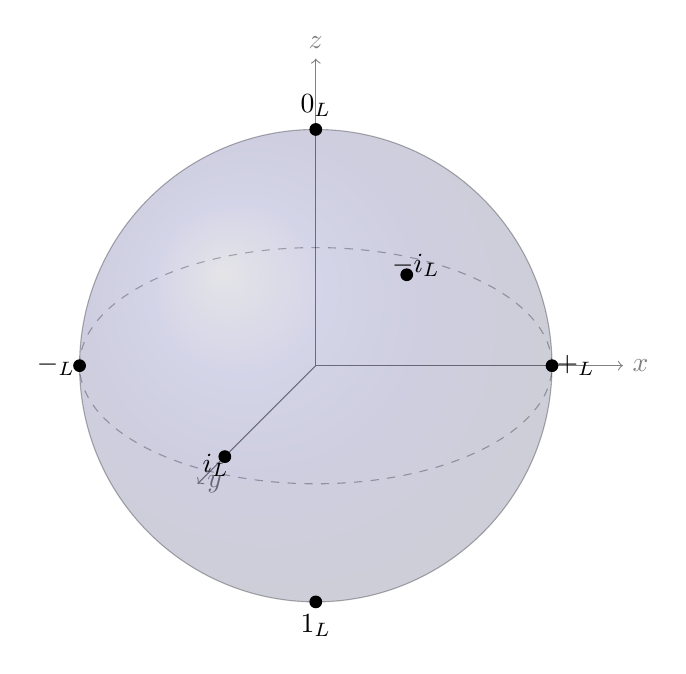
\begin{tikzpicture}[scale=3]
		% --- Ejes ---
		\draw[->, gray] (0,0,0) -- (1.3,0,0) node[anchor=west]{$x$};
		\draw[->, gray] (0,0,0) -- (0,1.3,0) node[anchor=south]{$z$};
		\draw[->, gray] (0,0,0) -- (0,0,1.3) node[anchor=west]{$y$};
		% --- Esfera ---
		\draw[black, opacity=0.3] (0,0) circle (1);
		\draw[dashed, opacity=0.3] (0,0) ellipse (1cm and 0.5cm);
		\fill[ball color=blue, opacity=0.1] (0,0) circle (1);
		% --- Polos (Estados Z) ---
		\node at (0, 1.1) {$\ket{0_L}$};
		\node at (0, -1.1) {$\ket{1_L}$};
		\draw[fill] (0,1) circle (0.7pt);
		\draw[fill] (0,-1) circle (0.7pt);
		% --- Eje X (Estados X) ---
		\node at (1.1, 0, 0) {$\ket{+_L}$};
		\node at (-1.1, 0, 0) {$\ket{-_L}$};
		\draw[fill] (1,0,0) circle (0.7pt);
		\draw[fill] (-1,0,0) circle (0.7pt);
		% --- Eje Y (Estados Y) ---
		\node at (0, 0, 1.1) {$\ket{i_L}$};
		\node at (0, 0, -1.1) {$\ket{-i_L}$};
		\draw[fill] (0,0,1) circle (0.7pt);
		\draw[fill] (0,0,-1) circle (0.7pt);
	\end{tikzpicture}
	\caption{La esfera de Bloch, mostrando la parametrización
		$(\theta, \phi)$ de un estado genérico $\ket{\psi}$ y la ubicación
	de los autoestados de $X_L$, $Y_L$ y $Z_L$.}
	\label{fig:bloch}
\end{figure}
\section{Conexión con la Ecuación de Schrödinger y Dinámica de Puertas}

\subsection{Ecuación de Schrödinger en el Subespacio Lógico}

La dinámica de cualquier estado cuántico $\ket{\psi(t)}$ está gobernada por
la ecuación de Schrödinger dependiente del tiempo:
%
$$
i\hbar \pdv_{t}\ket{\psi(t)} = \hat{H} \ket{\psi(t)}
$$
%
donde $\hat{H}$ es el Hamiltoniano total del sistema.

Nos interesa la dinámica \emph{restringida} al subespacio lógico
$\mathcal{H}_L = \text{span}\{\ket{0_L}, \ket{1_L}\}$.
Suponiendo que el sistema permanece confinado a este subespacio (es
decir, ignorando la fuga (leakage) a estados $n \ge 3$ ),
podemos proyectar el Hamiltoniano físico sobre esta base.

El Hamiltoniano de la partícula libre (sin perturbaciones externas) en el
pozo es $\hat{H}_0 = -\frac{\hbar^2}{2m}D_x^2 + V(x)$.
Los estados $\ket{0_L}$ y $\ket{1_L}$ son, por definición, autoestados
de $\hat{H}_0$ con autovalores $E_1$ y $E_2$ respectivamente
.

El Hamiltoniano efectivo para el sistema libre, $\hat{H}_{\text{free}}$,
actuando solo dentro de $\mathcal{H}_L$, se obtiene proyectando $\hat{H}_0$:
%
$$
\hat{H}_{\text{free}} = \hat{P}_L \hat{H}_0 \hat{P}_L
$$
%
donde $\hat{P}_L = \dyad{0_L} + \dyad{1_L}$ es el proyector sobre
$\mathcal{H}_L$. Los elementos de matriz de este Hamiltoniano son:
%
$$
\mel{j_L}{\hat{H}_0}{k_L} = E_k \braket{j_L}{k_L} = E_k \delta_{jk}
\quad \text{para } j,k \in \{0, 1\}
$$
%
Esto se debe a la ortonormalidad de la base. Por lo
tanto, el Hamiltoniano efectivo es diagonal en la base lógica:
%
$$
\hat{H}_{\text{free}} = E_1 \dyad{0_L} + E_2 \dyad{1_L}
$$
%
Y la ecuación de Schrödinger para un estado $\ket{\psi(t)} \in \mathcal{H}_L$
se convierte en:
%
$$
i\hbar \pdv{t}\ket{\psi(t)} = (E_1 \dyad{0_L} + E_2 \dyad{1_L}) \ket{\psi(t)}
$$

\subsection{Hamiltoniano Efectivo y Rotación en la Esfera de Bloch}

Podemos reescribir $\hat{H}_{\text{free}}$ en términos de los operadores
de Pauli $Z_L$ e $I_L$, usando las definiciones $Z_L = \dyad{0_L} - \dyad{1_L}$
 y $I_L = \dyad{0_L} + \dyad{1_L}$.
%
$$
\dyad{0_L} = \frac{1}{2}(I_L + Z_L) \quad \text{y} \quad
\dyad{1_L} = \frac{1}{2}(I_L - Z_L)
$$
%
Sustituyendo en $\hat{H}_{\text{free}}$:
%
$$
\hat{H}_{\text{free}} = E_1 \frac{1}{2}(I_L + Z_L) + E_2 \frac{1}{2}(I_L - Z_L)
$$
$$
\hat{H}_{\text{free}} = \frac{E_1 + E_2}{2} I_L + \frac{E_1 - E_2}{2} Z_L
$$
%
El operador de evolución temporal $U(t) = \exp(-i \hat{H}_{\text{free}} t / \hbar)$
es:
%
$$
U(t) = \exp\left( \frac{-i (E_1 + E_2) t}{2\hbar} \right) I_L 
       \exp\left( \frac{-i (E_1 - E_2) t}{2\hbar} Z_L \right)
$$
%
El primer término, $\exp(-i (E_1 + E_2) t / 2\hbar) I_L$, es una
\textbf{fase global}. No tiene consecuencias físicas medibles, ya que
el vector de estado en la esfera de Bloch es invariante bajo fases
globales.

El término físicamente relevante es el segundo. Definiendo la frecuencia
de transición (o frecuencia de Larmor del qubit) como
$\omega_{12} = (E_2 - E_1) / \hbar$, podemos reescribir el Hamiltoniano
físicamente relevante (ignorando la fase global) como:
%
$$
\hat{H}_{\text{eff}} = \frac{E_1 - E_2}{2} Z_L = -\frac{\hbar \omega_{12}}{2} Z_L
$$
%
El operador de evolución temporal (sin fase global) es:
%
$$
U_{\text{eff}}(t) = \exp\left( -i \hat{H}_{\text{eff}} t / \hbar \right) =
\exp\left( i \frac{\omega_{12} t}{2} Z_L \right)
$$
%
Este operador es, por definición, el operador de rotación alrededor
del eje $z$ de la esfera de Bloch por un ángulo $\theta_Z(t) = -\omega_{12} t$.
%
$$
U_{\text{eff}}(t) = R_Z(-\omega_{12} t)
$$
%
Esto demuestra que la \textbf{evolución libre} del qubit (cuando se deja
sin perturbar) es simplemente una rotación continua alrededor del eje $z$
a una velocidad constante $\omega_{12}$. Las poblaciones $|\alpha|^2$ y
$|\beta|^2$ (probabilidades de medir $E_1$ o $E_2$) permanecen constantes,
mientras que la fase relativa entre los dos estados evoluciona en el
tiempo. Esto es coherente con el hecho de que $\ket{0_L}$ y $\ket{1_L}$
son estados estacionarios (autoestados de energía).

\subsection{Interpretación como Puerta Cuántica}

La dinámica descrita por $U_{\text{eff}}(t)$ es en sí misma una
\textbf{puerta cuántica}. Si dejamos el sistema evolucionar libremente
durante un tiempo $t = \phi / (-\omega_{12})$, implementamos la
puerta $R_Z(\phi)$. Esta es una puerta de fase.

Sin embargo, para la computación cuántica universal, se requiere la
capacidad de implementar \emph{rotaciones arbitrarias} en la esfera de
Bloch, no solo rotaciones $R_Z$. Específicamente, se necesita control
sobre al menos un eje de rotación adicional (por ejemplo, $X_L$).

Esto se logra aplicando un Hamiltoniano de interacción externo
dependiente del tiempo, $\hat{H}_{\text{int}}(t)$. Como se discutió
previamente, la carga $q$ y el espín $s$ de la partícula proporcionan
los ``manejadores'' para este control.

Por ejemplo, la aplicación de un campo eléctrico externo $\vec{E}(t)$
 puede modular el potencial $V(x)$. Si este campo oscila a una
frecuencia $\omega$ cercana a la frecuencia de resonancia $\omega_{12}$,
inducirá transiciones entre $\ket{0_L}$ y $\ket{1_L}$. En el marco de la
aproximación de onda rotante (RWA), este Hamiltoniano de interacción,
visto en el marco giratorio, puede tomar la forma de:
%
$$
\hat{H}_{\text{RWA}} \propto \Omega X_L
$$
%
donde $\Omega$ es la frecuencia de Rabi, que es proporcional a la
amplitud del campo $\vec{E}$ aplicado.

La evolución bajo este Hamiltoniano, $U_X(t) = \exp(-i (\Omega' t) X_L)$,
corresponde a una \textbf{rotación alrededor del eje $x$}
(una puerta $R_X$).

Al tener la capacidad de generar rotaciones $R_Z$ (mediante la evolución
libre controlada por tiempos de espera) y rotaciones $R_X$ (mediante la
aplicación de campos resonantes), se puede construir cualquier
operación unitaria $U \in SU(2)$ (cualquier puerta de un solo qubit)
mediante la composición de estas rotaciones (por ejemplo, $U = R_Z(\phi_1)
R_X(\theta) R_Z(\phi_2)$).

Por lo tanto, la ``dinámica de puertas'' es la implementación de
operaciones $SU(2)$ deseadas mediante la conmutación controlada y
temporizada de Hamiltonianos de evolución libre ($\propto Z_L$) e
interacción ($\propto X_L$ o $Y_L$).
\section{Glosario}

A continuación, se definen los conceptos clave introducidos en el desarrollo del
trabajo.

\begin{description}
  \item[\textbf{Espacio de Hilbert ($\mathcal{H}$):}]
    Es un espacio vectorial complejo (donde viven los kets, $|\psi\rangle$)
    dotado de un producto interno, que además es completo. En mecánica cuántica,
    el conjunto de todos los posibles estados de un sistema físico forma un
    espacio de Hilbert.

  \item[\textbf{Producto Interno:}]
    Es una función (denotada $\langle \cdot, \cdot \rangle$) que toma dos
    vectores de un espacio vectorial $V$ y devuelve un escalar en el campo $F$
    sobre el cual $V$ está definido (usualmente $\mathbb{R}$ o $\mathbb{C}$).
    Esta función debe satisfacer propiedades específicas: ser positiva-definida,
    tener simetría conjugada ($\langle v, w \rangle = \langle w, v \rangle^*$) y
    ser lineal en uno de sus argumentos (en mecánica cuántica, por convención,
    es lineal en el segundo argumento, el ket). En el contexto de un espacio de
    Hilbert complejo ($\mathbb{C}$), el producto interno
    $\langle\phi|\psi\rangle$ devuelve un número complejo. Su propósito es
    definir la geometría del espacio, permitiendo calcular normas ($\|\psi\|^2 =
    \langle\psi|\psi\rangle$), probabilidades y verificar la ortogonalidad
    ($\langle\phi|\psi\rangle = 0$).

  \item[\textbf{Estado Propio (Autoestado):}]
    Un vector $|\psi\rangle$ (distinto de cero) que, al ser actuado por un
    operador $\hat{A}$, no cambia su ``dirección'' en el espacio de Hilbert,
    sino que solo es multiplicado por un escalar $a$, llamado autovalor.
    Satisface la ecuación de autovalores $\hat{A}|\psi\rangle = a|\psi\rangle$.
    Los estados estacionarios $\psi_n$ son autoestados del Hamiltoniano
    $\hat{H}$.

  \item[\textbf{Superposición Lineal:}]
    Matemáticamente, es un sinónimo de combinación lineal. Es una expresión
    formada por la suma de vectores de un espacio vectorial (como los kets
    $|\psi_1\rangle, |\psi_2\rangle$), donde cada vector es multiplicado por un
    coeficiente escalar (como $\alpha, \beta \in \mathbb{C}$). La forma general
    es $|\Psi\rangle = \alpha|\psi_1\rangle + \beta|\psi_2\rangle$. El Principio
    de Superposición es el postulado fundamental de la mecánica cuántica que
    establece que si $|\psi_1\rangle$ y $|\psi_2\rangle$ son estados válidos de
    un sistema, cualquier superposición lineal de ellos (con $|\alpha|^2 +
    |\beta|^2 = 1$) también es un estado físico válido, que existe como una
    combinación de ambos hasta que se realiza una medición.

  \item[\textbf{Base Lógica:}]
    Un conjunto de estados ortonormales ($\{|0_L\rangle, |1_L\rangle\}$)
    elegidos de un espacio de Hilbert para representar bits de información. Se
    les llama ``lógicos'' o ``computacionales'' porque abstraen la física
    subyacente (en este caso, los niveles de energía) a los conceptos de 0 y 1.

  \item[\textbf{Qubit (Qubit Lógico):}]
    La unidad básica de información cuántica. Es un sistema cuántico de dos
    niveles (como los dos estados de energía $\psi_1, \psi_2$) cuya base lógica
    es $|0_L\rangle$ y $|1_L\rangle$. Su estado general es una superposición
    lineal $|\psi\rangle = \alpha|0_L\rangle + \beta|1_L\rangle$.

  \item[\textbf{Observable:}]
    Cualquier propiedad física de un sistema que, en principio, puede ser medida
    (ej. energía, posición, momento, espín). En el formalismo cuántico, cada
    observable está representado por un operador hermítico. Los resultados de
    una medición solo pueden ser los autovalores de dicho operador.

  \item[\textbf{Operador Hermítico:}]
    Un operador $\hat{A}$ que es igual a su propio adjunto (conjugado
    transpuesto), es decir, $\hat{A} = \hat{A}^\dagger$. Son fundamentales
    porque garantizan dos cosas: 1) Sus autovalores son siempre números reales
    (lo cual es necesario, ya que las mediciones dan resultados reales). 2) Sus
    autoestados forman una base ortonormal para el espacio de Hilbert.

  \item[\textbf{Producto Tensorial ($\otimes$):}]
    Es una operación algebraica que construye un nuevo espacio vectorial
    $\mathcal{H}_{AB} = \mathcal{H}_A \otimes \mathcal{H}_B$ a partir de dos
    espacios $\mathcal{H}_A$ y $\mathcal{H}_B$. Si $\dim(\mathcal{H}_A) = n$ y
    $\dim(\mathcal{H}_B) = m$, entonces $\dim(\mathcal{H}_{AB}) = n \times m$.
    Físicamente, es la operación matemática que permite construir el espacio de
    Hilbert de un sistema compuesto a partir de los espacios de sus subsistemas
    (ej. $\mathcal{H}_{total} = \mathcal{H}_L \otimes \mathcal{H}_{spin}$). Un
    estado en este espacio combinado especifica el estado de todas sus partes
    simultáneamente y permite la existencia del entrelazamiento.

  \item[\textbf{Espín:}]
    Una forma intrínseca de momento angular que posee una partícula (como el
    electrón). Es una propiedad puramente cuántica, sin un análogo clásico
    directo, que se describe como un grado de libertad interno de la partícula
    (ej. ``arriba'' $|\uparrow\rangle$ y ``abajo'' $|\downarrow\rangle$ para una
    partícula de espín $s=1/2$).

  \item[\textbf{Operadores de Pauli:}]
    Un conjunto de tres operadores hermíticos ($X_L, Y_L, Z_L$) que son
    fundamentales para describir la dinámica y los observables de un sistema de
    dos niveles (qubit). Físicamente, están relacionados con las mediciones del
    espín en las tres direcciones espaciales (x, y, z) y matemáticamente forman
    una base para los operadores del qubit.

  \item[\textbf{Entrelazamiento:}]
    Un fenómeno puramente cuántico que describe una correlación entre dos o más
    sistemas (como qubits) que no puede existir en la física clásica. Un sistema
    compuesto se dice entrelazado si su estado cuántico total no puede ser
    factorizado o descrito como una simple combinación de los estados
    individuales de sus subsistemas (es decir, no es un estado separable). Como
    resultado, una medición realizada sobre uno de los sistemas parece influir
    instantáneamente en el resultado de la medición sobre el otro, sin importar
    la distancia que los separe.

  \item[\textbf{Regla de Born:}] Postulado fundamental que conecta el formalismo
    matemático del vector de estado $\ket{\psi}$ con los resultados de una
    medición. Si un sistema se mide en una base ortonormal $\{\ket{\phi_i}\}$,
    la probabilidad de obtener el resultado asociado al autoestado $\ket{\phi_i}$
    es $P(i) = |\braket{\phi_i}{\psi}|^2$.

  \item[\textbf{Esfera de Bloch:}] Representación geométrica del espacio de estados
    puros de un qubit (un sistema de dos niveles) $\mathcal{H}_L$. Cada
    estado $\ket{\psi} = \cos(\theta/2)\ket{0_L} + e^{i\phi}\sin(\theta/2)\ket{1_L}$
    se mapea a un punto único en la superficie de una esfera de radio unidad
    mediante los ángulos $(\theta, \phi)$. Los estados ortogonales ocupan puntos
    antipodales.

  \item[\textbf{Puerta cuántica:}] Operación fundamental que transforma el estado de
    un qubit. Matemáticamente, se describe como una \emph{rotación unitaria} $U$
    (un operador en $SU(2)$) que actúa sobre el vector de estado en la esfera
    de Bloch. Físicamente, se implementa mediante la evolución temporal
    $U(t) = \exp(-i\hat{H}_{\text{eff}}t/\hbar)$ bajo un Hamiltoniano efectivo
    $\hat{H}_{\text{eff}}$ aplicado de forma controlada.

  \item[\textbf{Medida computacional:}] Proceso de medición de un qubit en la base
    lógica (o computacional) $\{\ket{0_L}, \ket{1_L}\}$. Corresponde a medir el
    observable $Z_L = \dyad{0_L} - \dyad{1_L}$. En el sistema físico del pozo
    de potencial, esta medición es físicamente equivalente a medir la energía
    (distinguiendo entre $E_1$ y $E_2$).

  \item[\textbf{Hamiltoniano efectivo:}] Operador que describe la dinámica de un
    sistema restringido a un subespacio de interés (como el subespacio lógico
    $\mathcal{H}_L$). Se obtiene proyectando el Hamiltoniano físico completo
    $\hat{H}$ sobre dicho subespacio ($\hat{H}_{\text{eff}} =
    \hat{P}_L \hat{H} \hat{P}_L$) y, comúnmente, omitiendo términos que solo
    contribuyen a una fase global, como los proporcionales al operador
    identidad $I_L$.

  \item[\textbf{Rotación unitaria:}] Transformación lineal $U$ en un espacio de Hilbert
    que preserva el producto interno (y, por tanto, la norma de los vectores y
    la probabilidad total). Satisface la condición $U^\dagger U = I$. Según la
    ecuación de Schrödinger, la evolución temporal de cualquier sistema cuántico
    cerrado es una rotación unitaria. Las puertas cuánticas son
    implementaciones físicas de rotaciones unitarias específicas.

  \item[\textbf{Subespacio invariante:}] Subespacio vectorial
    $\mathcal{S} \subseteq \mathcal{H}$ tal que, al aplicar un operador $\hat{A}$,
    todos los vectores de $\mathcal{S}$ se transforman en vectores que también
    pertenecen a $\mathcal{S}$ (es decir, $\hat{A}\ket{\psi} \in \mathcal{S}$
    para todo $\ket{\psi} \in \mathcal{S}$). En el diseño de un qubit lógico,
    el objetivo es que el subespacio $\mathcal{H}_L$ sea invariante bajo la
    evolución temporal $U(t)$ de las puertas, evitando la fuga (leakage) a
    estados fuera del subespacio computacional.

  \item[\textbf{Coherencia cuántica:}] Propiedad de un sistema cuántico para mantener
    una superposición de estados con una relación de fase relativa definida,
    como en $\ket{\psi} = \alpha\ket{0_L} + \beta\ket{1_L}$.
    La coherencia es la responsable de los términos de interferencia.
    Matemáticamente, la coherencia se cuantifica por los elementos fuera de la
    diagonal de la matriz de densidad $\rho$. La pérdida de esta relación de fase
    (decoherencia) destruye la superposición y la interferencia.
\end{description}
